\chapter{Multi-precision Addition}

\section{Theory of Addition}
\defbox[$n$-bit string]{\begin{definition}
	A positive integer $X\in\Z^+$ is a $n$-bit string if and only if \[
	2^{n-1}\leq X<2^n.
	\]
\end{definition}}
\begin{remark}
A positive integer $X\in\Z^+$ is a $n$-word string if and only if \[
(2^w)^{n-1}\leq X<(2^w)^n.
\] In computing, word lengths of 8, 32, and 64 bits are generally used. That is, \[
w\in\set{8,32,64}.
\]
\end{remark}
\vfill
\begin{example}
	Let $n=wt$ with $w=32$ and $t=4$. Consider 4-word string $X=\sum_{i=0}^{t-1}x_i(2^w)^i$: \begin{align*}
	\sum_{i=0}^{3}x_i(2^w)^i&=x_3\cdot 2^{3w}+x_2\cdot 2^{2w}+x_1\cdot 2^{w}+x_0\\
	&=x_3\cdot 2^{96}+x_2\cdot 2^{64}+x_1\cdot 2^{32}+x_0,
	\end{align*} where $x_0\in\intco{0,2^w}$ for $i=0,1,2,3$. That is:
	\begin{center}
		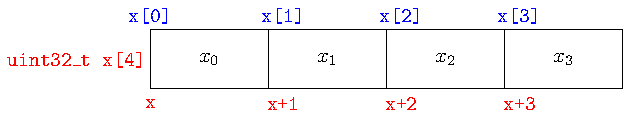
\includegraphics[]{tikz/example1-1.pdf}
	\end{center}
	If $w=32$ (\texttt{uint32\_t}), then \begin{table}[h!]\centering\renewcommand{\arraystretch}{1.25}
		{\ttfamily\begin{tabular}{c|c|c|c|c|l}
				\cline{2-5}
				\textnormal{\bf Minimum} & 00000001 & 00000000 & 00000000 & 00000000 & $=2^{3w}=2^{96}$\\ \cline{2-5}
				\textnormal{\bf Maximum} & FFFFFFFF & FFFFFFFF & FFFFFFFF & FFFFFFFF & $=2^{4w}-1=2^{128}-1$\\ \cline{2-5}
		\end{tabular}}
	\end{table}
\end{example}

\newpage
\probox[Memory Limits in Multi-Precision Addition]{\begin{proposition}
	Let $X$ and $Y$ are $n$-word and $m$-word strings, respectively, that is,
	\begin{align*}
		(2^w)^{n-1}&\leq X<(2^w)^n,\\
		(2^w)^{m-1}&\leq Y<(2^w)^m.
	\end{align*} Then \[
	(2^w)^{\max(n,m)-1}< X<(2^w)^{\max(n,m)+1}.
	\]
\end{proposition}}
\begin{proof}
	Two integers $X$ and $Y$ can be expressed as follows: \begin{align*}
		X&=q_x(2^w)^{n-1}+r_x\quad\text{and}\\
		Y&=q_y(2^w)^{m-1}+r_y,
	\end{align*} where \[
	0< q_x,q_y< 2^w,\quad
	0\leq r_x< (2^w)^n,\quad
	0\leq r_y< (2^w)^m.
	\] If $n\geq m$ then \begin{align*}
	(2^w)^{n-1}\leq\max(X,Y)<X+Y&=
\end{align*}
\end{proof}

\probox[Sing-word Addition]{\begin{proposition}
	Let $X,Y$ be single-word strings, that is, \[
	0\leq X,Y<2^w.
	\] \begin{enumerate}[(1)]
		\item \begin{align*}
		X+Y&=\floor*{\frac{X+Y}{2^w}}2^w+(X+Y\bmod 2^w) \\
		&=\floor*{\frac{X+Y}{2^w}}2^w+(X\boxplus_{32} Y).
		\end{align*}
		\item {\normalfont (carry)} $\floor*{\frac{X+Y}{2^w}}\in\set{0,1}$
		\item $0\leq X+Y<2^{2w}$.
		\item $\floor*{\frac{X+Y}{2^w}}=1\iff 2^w\leq X+Y\iff (X\boxplus_{32} Y)<X$.
	\end{enumerate}
\end{proposition}}
\begin{proof}
	content...
\end{proof}

\section{Implementation of Multi-precision Addition}

\begin{algorithm}[H]
	\DontPrintSemicolon
	\caption{Multi-Precision Addition}
	\KwIn{$X,Y\in\intco{0,2^{wt}}$\tcp*{$X=\sum_{i=0}^{t-1}(x_i\cdot 2^w)$ and $Y=\sum_{j=0}^{t-1}(y_j\cdot 2^w)$ with $x_i,y_j\in\intco{0,2^w}$}}
	\KwOut{$(\varepsilon,Z)$ where $Z=X+Y\bmod 2^{wt}$ with carry bit $\varepsilon$\tcp*{$Z=\sum_{k=0}^{t}(x_k+y_k+\varepsilon)$ and $\varepsilon\in\set{0,1}$}}
	\BlankLine
	$(\varepsilon,z[0])\gets x[0]+y[0]$\;
	\For{$i=1$ \KwTo $t-1$}{
		$(\varepsilon,z[i])\gets x[i] + y[i] + \varepsilon$\;
	}
	\Return $(\varepsilon, Z)$\tcp*{$Z=\sum_{i=0}^{t-1}(z_i\cdot2^w)=z[t-1]\adjacent z[t-2]\adjacent\cdots\adjacent z[0]$}
\end{algorithm}
\begin{example}
\ \begin{table}[h!]\centering\renewcommand{\arraystretch}{1.25}
{\ttfamily\begin{tabular*}{\textwidth}{@{\extracolsep{\fill}}cccccc}
	$X$ & & 0xFFFFFFFF & 0xFFFFFFFF & 0xFFFFFFFF & 0xFFFFFFFF \\
	$Y$ & + & 0xFFFFFFFF & 0xFFFFFFFF & 0xFFFFFFFF & 0xFFFFFFFF \\
	\color{red} $\varepsilon$ & \color{red}0x00000001 & \color{red}0x00000001 & \color{red}0x00000001 & \color{red}0x00000001 & \color{red}0x00000000 \\ \cline{2-6}
	$Z$ & 0x00000001 & 0xFFFFFFFF & 0xFFFFFFFF & 0xFFFFFFFF & 0xFFFFFFFE \\
\end{tabular*}}
\end{table}
\end{example}
\begin{lstlisting}[style=normal]
CARRY
BN_ADD(digit_t* ret, digit_t* opA, digit_t* opB, digit_t len) {
	COUNT cnt_i;
	digit_t carry = 0; 			// for option 1, 2, 3
	digit_t tmp = 0; 			// for option 1
	dbl_digit_t accu = 0x00; 	// for option 3
	
	// Option 1
	for (cnt_i = 0; cnt_i < len; cnt_i++) {
		tmp = opA[cnt_i];
		tmp += carry;
		carry = (tmp < carry);
		temp += opB[cnt_i];
		carry += (tmp < opB[cnt_i]);
		ret[cnt_i] = tmp;
	}
	return carry;
}
\end{lstlisting}
\begin{lstlisting}[style=normal]
uint32_t bn_add_c(uint64_t* ret, uint64_t* opA, uint64_t* opB, int32_t len) {
	int32_t cnt_i;
	uint64_t carry = 0, temp = 0;
	
	for(cnt_i = 0; cnt_i < len; cnt_i++) {
		temp = opA[cnt_i];
		temp += carry;
		carry = (temp < carry);
		temp += opB[cnt_i];
		carry += (temp < opB[cnt_i]);
		ret[cnt_i] = temp;
	}
	return carry;
}
\end{lstlisting}

\begin{lstlisting}[style=normal]
void addition_single(word* epsilon, word* dst, const word src1, const word src2) {
	word tmp = *epsilon;
	word sum = src1 + src2;
	*epsilon = (sum < src1); 		// Set epsilon to 1 if there was a carry-out, otherwise 0
	sum += tmp; 					// Add epsilon (this will be either 0 or 1)
	*epsilon += (sum < *epsilon); 	// Adjust epsilon if there was a carry-out from this addition
	*dst = sum; 					// Set the destination word
}
\end{lstlisting}
